\documentclass[pdf]{beamer}
\usetheme{AnnArbor}         % tema
\usecolortheme{orchid}      % cores
\mode<presentation>{}
\usepackage{multirow}
\usepackage{hyperref}
\usepackage{color}
\usepackage{epsfig}
\usepackage{amsthm}
\usepackage{amssymb}
\usepackage{amsmath}
\usepackage{amscd}
\usepackage[brazilian]{babel}
%\usepackage[utf8]{inputenc}
\usepackage{float}
\usepackage{algpseudocode}
\usepackage{subfig}
\usepackage{listings}
\usepackage{tikz}


\DeclareMathOperator*{\argmin}{arg\,min}
\DeclareMathOperator*{\argmax}{arg\,max}
\algnewcommand{\LineComment}[1]{\State \(\triangleright\) #1}
\def  \R   {{\mathbb R}}
\def  \Z   {{\mathbb Z}}
%\def  \N   {{\mathbb N}}
\def  \Q   {{\mathbb Q}}
\def \Ev {{\mathbb E}}
\def \Pr {{\mathbb P}}
\def \f {{\mathbf f}}
\def \u {{\mathbf u}}
\def \y {{\mathbf y}}
\def \x {{\mathbf x}}
\def \m {{\mathbf m}}
\def \gu {{\bar{g}}}

\newcommand{\Var}{\mathrm{Var}}
\newcommand{\Cov}{\mathrm{Cov}}

%% preamble
\title{The title}
\subtitle{The subtitle}
\author{your name}
\begin{document}

\lstset{frame=tb,
	language=Python,
	aboveskip=3mm,
	belowskip=3mm,
	showstringspaces=false,
	columns=flexible,
	basicstyle={\small\ttfamily},
	numbers=none,
	numberstyle=\tiny\color{gray},
	keywordstyle=\color{blue},
	commentstyle=\color{dkgreen},
	stringstyle=\color{mauve},
	breaklines=true,
	breakatwhitespace=true,
	tabsize=3
}

{\setbeamertemplate{footline}{} 
	\frame{\titlepage}}

\section*{Outline}\begin{frame}{Outline}\tableofcontents
\end{frame}
%% title frame
\begin{frame}
\titlepage
\end{frame}

%% normal frame
\section{Introduction}
\begin{frame}{Introduction}
Some introduction.
\end{frame}

\begin{frame}{Introduction}
\begin{block}{Bayesian theory}
Building blocks
\begin{itemize}
	\item Prior probability $p(\theta)$
	\item Likelihood $p(\mathcal{D}|\theta)$
\end{itemize}

Posterior probability
\begin{equation*}
 p(\mathcal{\theta}|\mathcal{D}) = \frac{p(\mathcal{D}|\theta) p(\theta)}{\int p(\mathcal{D}|\theta') p(\theta') d \theta'}
\end{equation*}
\pause
Using posterior probability:
\begin{equation*}
\int_\Theta f(\theta) p(\theta|\mathcal{D},M) d \theta
\end{equation*}
\end{block}
\pause
\begin{block}{}
	\centering{\textbf{Bayesian theory requires integration!}}
\end{block}

\end{frame}


\begin{frame}{Introduction}
\begin{block}{Approximate inference}
Ways to integrate:
\begin{itemize}
	\item Monte Carlo
	\begin{equation*}
	\int_\Theta f(\theta) p(\theta|\mathcal{D}) d\theta \approx \frac{1}{N} \sum_{i=1}^N f(\theta_i), \, \theta_i \sim p(\theta|\mathcal{D})
	\end{equation*}
	\item Approximate distribution
	\begin{equation*}
	p(\theta|\mathcal{D}) \approx q(\theta), \quad \int_\Theta  f(\theta) q(\theta) d\theta
	\end{equation*}
\end{itemize}

\pause
\begin{block}{}
\centering{Usual methods demands many evaluations of $p(\mathcal{D}|\theta) p(\theta)$. However, \textit{this is not always feasible.}}
\end{block}

\end{block}
\end{frame}

\begin{frame}
\begin{block}{}
In science, there are many cases that $p(\mathcal{D}|\theta)$ demands the computation of a forward model $g(\theta)$, which comes from an expensive simulation.
  \begin{figure}[h]
	\centering
	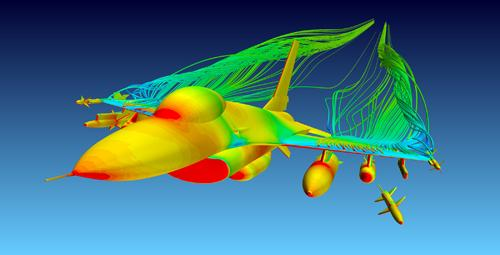
\includegraphics[height=0.3\paperheight]{figs/simulation_figure.jpg}
	%\includegraphics[height=6cm]{figCoordEsf02}
\end{figure}
\pause
This requires approximate inference methods "on a budget". In this work, one such method is developed, based on preexisting work. We name it
\pause 
\begin{block}{}
\centering{\textit{Boosted Variational Bayesian Monte Carlo (BVBMC)}.}
\end{block}
\end{block}
\end{frame}

\begin{frame}{Introduction}
\begin{block}{BVBMC schema}
  \begin{figure}[h]
	\centering
	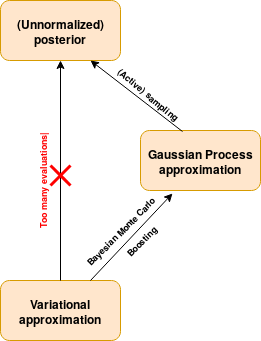
\includegraphics[height=.5\linewidth]{figs/diagram1a.png}
	%\includegraphics[height=6cm]{figCoordEsf02}
\end{figure}
\end{block}
\end{frame}
\begin{frame}{Introduction}
\begin{block}{An illustration of BVBMC}
	\centering{
	 \begin{tikzpicture}
	\node<1> (exfig1) {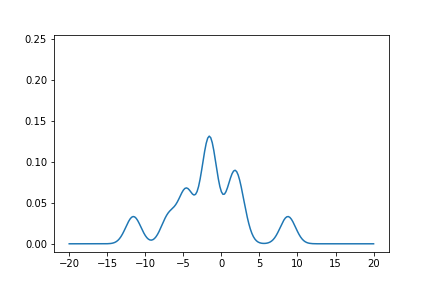
\includegraphics[width=.7\linewidth]{figs/exampleintro1}};
	\node<2> (exfig2) {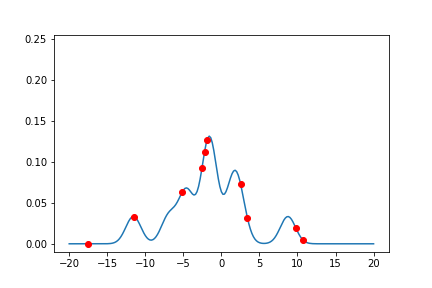
\includegraphics[width=.7\linewidth]{figs/exampleintro2}};
	\node<3> (exfig3) {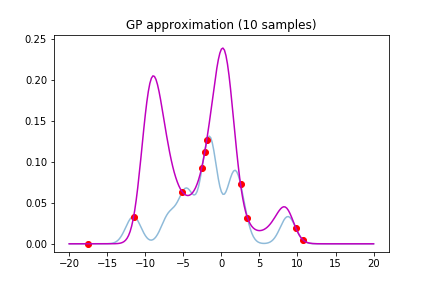
\includegraphics[width=.7\linewidth]{figs/exampleintro3}};
	\node<4> (exfig3) {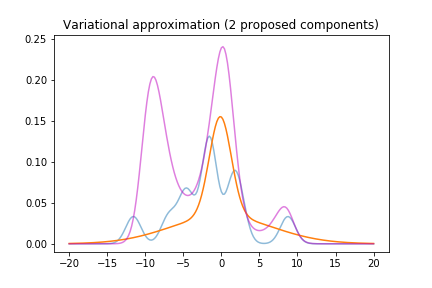
\includegraphics[width=.7\linewidth]{figs/exampleintro4}};
	\node<5> (exfig3) {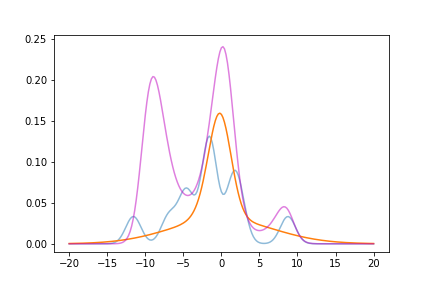
\includegraphics[width=.7\linewidth]{figs/exampleintro5}};
	\node<6> (exfig3) {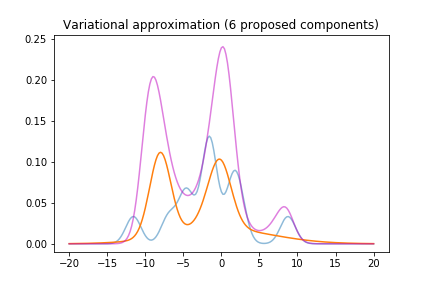
\includegraphics[width=.7\linewidth]{figs/exampleintro6}};
	\node<7> (exfig3) {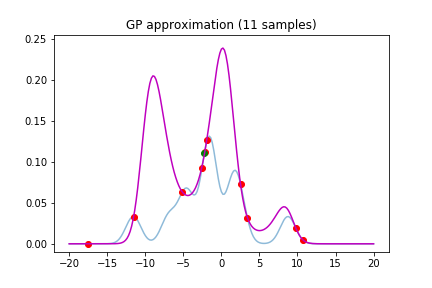
\includegraphics[width=.7\linewidth]{figs/exampleintro7}};
	\node<8> (exfig3) {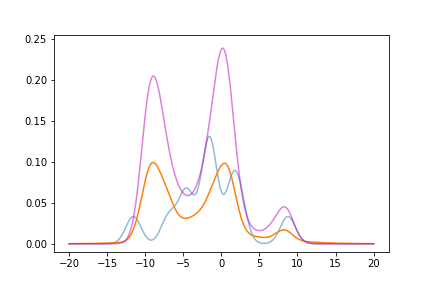
\includegraphics[width=.7\linewidth]{figs/exampleintro8}};
	\node<9> (exfig3) {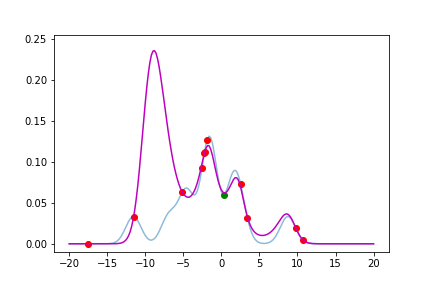
\includegraphics[width=.7\linewidth]{figs/exampleintro9}};
	\node<10> (exfig3) {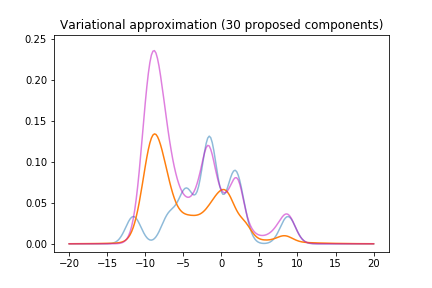
\includegraphics[width=.7\linewidth]{figs/exampleintro10}};
	\node<11> (exfig3) {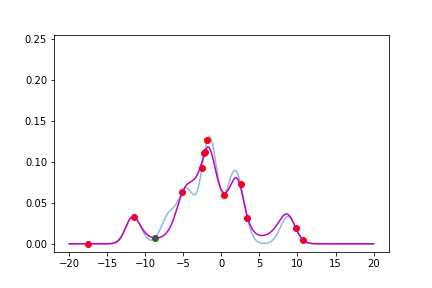
\includegraphics[width=.7\linewidth]{figs/exampleintro11}};
	\node<12> (exfig3) {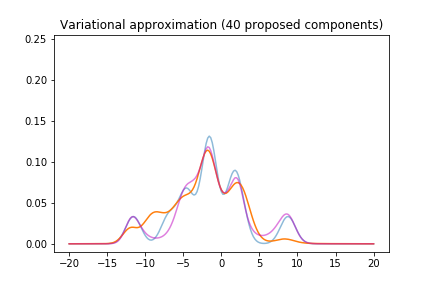
\includegraphics[width=.7\linewidth]{figs/exampleintro12}};
	\node<13> (exfig3) {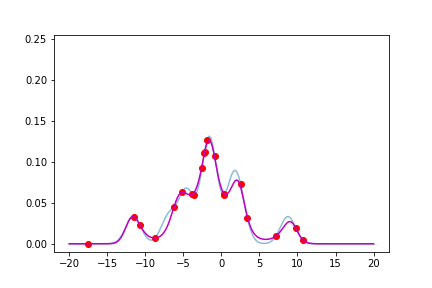
\includegraphics[width=.7\linewidth]{figs/exampleintro13}};
	\node<14> (exfig3) {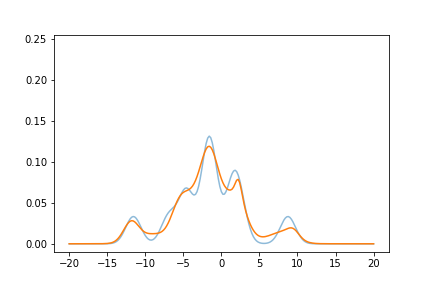
\includegraphics[width=.7\linewidth]{figs/exampleintro14}};

	\end{tikzpicture}
}
\end{block}
\end{frame}

\section{Gaussian Processes}
\begin{frame}{Gaussian Processes}
\begin{block}{Definition}
Gaussian processes (GP): distribution over functions $f:\mathcal{X} \to \mathbb{R}$ such that $f(\mathbf{x}) = (f(x_1),\ldots,f(x_n))$ follows a multivariate normal distribution. A GP is completely defined by:
\begin{itemize}
	\item $m(x) := \Ev[f(x)]$, mean function.
	\item $k(x,x') := \Ev[f(x),f(x')]$, covariance function or kernel.
\end{itemize}
such that $f(\mathbf{x}) \sim \mathcal{N}(m(\mathbf{x}),K(\mathbf{x},\mathbf{x}))$.
\end{block}
\pause
\begin{block}{Gaussian process regression}
Given $\mathcal{D} = {(x,y)}_{i=1}^N$, a Gaussian process regression is made by assuming $p(y|x) = p(y|f(x))$, with $f$ following a prior $GP(m,k)$.
\end{block}

\end{frame}

\begin{frame}{Gaussian Processes}
\begin{block}{Posterior GP}
If $p(y|f(x)) = \mathcal{N}(f(x),\sigma_n^2)$, $f|\mathcal{D} \sim GP(m_\mathcal{D},k_\mathcal{D})$, where 
\begin{equation*}
\begin{split}
 m_\mathcal{D}(x) & := m(x) + K(x^\star,\mathbf{x}) (K(\mathbf{x},\mathbf{x})+\sigma^2_n)^{-1} (\mathbf{y} - m(\mathbf{x})) \\
 k_\mathcal{D}(x,x') & := k(x,x') - K(x,\mathbf{x})(K(\mathbf{x},\mathbf{x})+\sigma_n^2)^{-1}K(\mathbf{x},x)
\end{split}
\end{equation*}
Reduces to deterministic measurement when $\sigma_n^2 = 0$. More general $p(y|f(x))$ must resort to explicit marginalization.
\end{block}
\end{frame}

\begin{frame}{Gaussian Processes}
\begin{block}{Example case}


\begin{figure}
	\centering
	\subfloat[GP prior]{\label{gprex1a}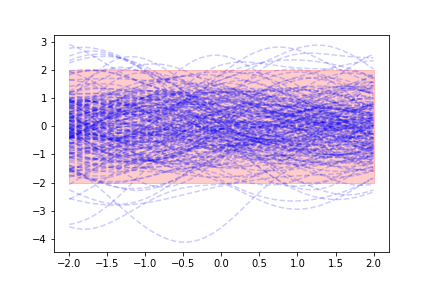
\includegraphics[width=0.5\textwidth]
		{figs/gprex1a.png}}
	\subfloat[GP posterior]{\label{gprex1b}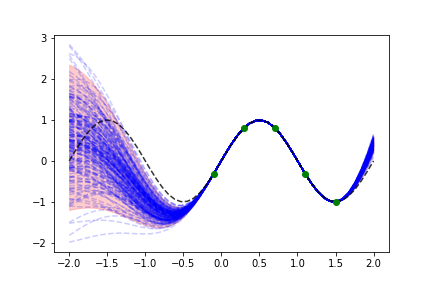
\includegraphics[width=0.5\textwidth]
		{figs/gprex1b.png}}

\end{figure}

\end{block}
\end{frame}

\begin{frame}{Gaussian Processes}
\begin{block}{Kernels}
The exigence that $K(\mathbf{x},\mathbf{x})$ limits which functions can be kernels. Some examples of kernels in $\mathbb{R}$ are:
\begin{itemize}
	\item $k_{SQE}(x,x') = \theta_0 \exp \left(-\frac{1}{2} \frac{(x-x')^2}{l^2} \right)$
	\item $k_{\text{Matern},3/2}(x,x') = \theta_0 \left( \sqrt{3} \frac{(x-x')}{l} \right) \exp \left(-\sqrt{3} \frac{(x-x')}{l}\right)$
\end{itemize}
Kernels in $\mathbb{R}^D$ can be constructed by changing $\frac{(x-x')}{l}$ for $\sqrt{\sum_{i=1}^D \frac{(x_i-x_i')}{l_i}}$.

If $k_1$,$k_2$ are kernels, the following, among others are kernels: $k_1(x,x')+k_2(x,x')$,$k_1(x,x')k_2(x,x')$,$k_1(x,x')k_2(y,y')$,$k_1(f(y),f(y'))$.
\end{block}
\pause
\begin{block}{Mean functions}
In general,they are less important than kernels, since the latter determines the structure of the posterior GP. However, \textit{outside the sampling area the GP prediction defaults to the mean}, which may be of importance.
\end{block}
\end{frame}

\begin{frame}{Gaussian processes}
\begin{block}{Handling hyperparameters}
\begin{equation*}
\begin{split}
\log p(\mathcal{D}|M,\sigma_n) = & -\frac{1}{2}(\mathbf{y} - m(\mathbf{x}))^T (K(\mathbf{x},\mathbf{x}) + \sigma_n \mathbf{I})^{-1} (\mathbf{y} - m(\mathbf{x})) + \\
&-\frac{1}{2} \log \det (K(\mathbf{x},\mathbf{x}) + \sigma_n \mathbf{I}) - \frac{1}{2} N \log(2\pi).
\end{split}
\end{equation*}
Inference can be done either by MLE, MAP, or integration techniques.
\end{block}
\begin{block}{Scaling}
The bottleneck of GP regression: $(K(\mathbf{x},\mathbf{x}) + \sigma_n \mathbf{I})^{-1}$. Cost is $\mathcal{O}(N^3)$.

In online learning, each new sample is incorporated in $\mathcal{O}(N^2)$.
\end{block}

\end{frame}

\section{Bayesian Monte Carlo}
\begin{frame}{Bayesian Monte Carlo}
\begin{block}{Integrating a GP}
\begin{equation*}
 Z = \int f(x) p(x) dx
\end{equation*}
If $f \sim GP(m,k)$, given $\mathcal{D} = \{(x_i,f(x_i))\}_{i=1}^N$, $Z_\mathcal{D} = \int f_\mathcal{D}(x) p(x) dx$ is Gaussian:
\begin{equation*}
\begin{split}
& \Ev[Z_{\mathcal{D}}] = \int m(x) p(x) dx - \mathbf{z}^T K^{-1} (\mathbf{f}-m(\mathbf{x})), \quad
\Var[Z_{\mathcal{D}}] = \Gamma - \mathbf{z}^T K^{-1} \mathbf{z}, \\
& z_i = \int k(x,x_i) p(x) dx, \quad \Gamma = \int \int k(x,x') p(x) p(x') dx dx'.
\end{split}
\end{equation*}
\pause
\begin{block}{}
\centering{Name Bayesian \textit{Monte Carlo} is misleading.}
\pause

\centering{Treating $f$ as a random variable may be philosophically odd.}
\end{block}
\end{block}
\end{frame}
\begin{frame}{Bayesian Monte Carlo}
\begin{figure}
	\centering
	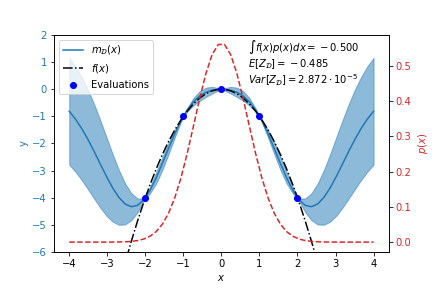
\includegraphics[width=0.8\linewidth]{figs/exbmc.png}
\end{figure}
\end{frame}
\begin{frame}{Bayesian Monte Carlo}
\begin{block}{Kernel integral terms}
In the general case, they can be estimated by Monte Carlo.
When $p(x)$ is Gaussian or a mixture of Gaussians:
\begin{itemize}
	\item Analytically tractable when $k(x,x')$ is the SQE kernel.
	\item Efficiently tractable when $k(x,x') = k(x_1,y_1) \ldots k(x_D,y_D)$.
\end{itemize}
\begin{block}{Active sampling}
	Given $\{(x_1,f(x_1),\ldots,x_N,f(x_N)\}$, $x_{N+1}$ may be chosen by optimizing acquisition functions.
\begin{equation*}
\alpha^N_{\text{MMLT}}(x) = e^{2 m_\mathcal{D}(x) + k_\mathcal{D}(x,x)} \left(e^{k_\mathcal{D}(x,x)}-1\right).
\end{equation*}
\end{block}
\end{block}
\end{frame}

\section{Variational Inference}
\begin{frame}{Variational Inference}
\begin{block}{Back to approximating posteriors $p(\theta|\mathcal{D}) \approx q(\theta;\lambda)$}

Variational Inference: given $g(\theta)$, seeks minimization of $D_{KL}(q(\cdot;\lambda)||g)$.

Given unnormalized $\gu$, this is equivalent to maximizing the evidence lower bound (ELBO) 
\begin{equation*}
\mathcal{L}(\lambda) = 
\int \log \gu(\theta) q(\theta) d\theta - \int \log q(\theta) q(\theta) d\theta
\end{equation*}
The family of variational posteriors $q(\theta;\lambda)$ must be easy to treat, in order for the approximation to be useful.


\end{block}
\begin{block}{$D_{KL}(q(\cdot;\lambda)||g)$ vs $D_{KL}(g||q(\cdot;\lambda))$}
$D_{KL}(q(\cdot;\lambda)||g) \neq D_{KL}(g||q(\cdot;\lambda))$: two minimization objectives. Gives two different algorithms (the second one, \textit{expectation propagation}, is not treated here).

\end{block}
\end{frame}

\begin{frame}{Variational Inference}
\begin{block}{Illustration}
\begin{figure}
	\centering
	\subfloat[$D_{KL}(q||g)$ ]{\label{vixep1a}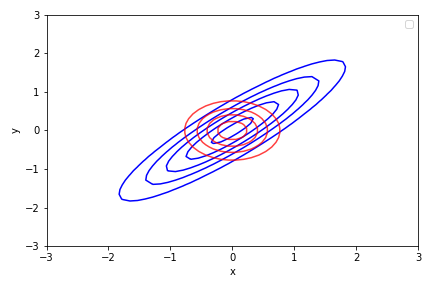
\includegraphics[width=0.45\textwidth]
		{figs/klil3a.png}}
	\subfloat[$D_{KL}(g||q)$]{\label{vixep1b}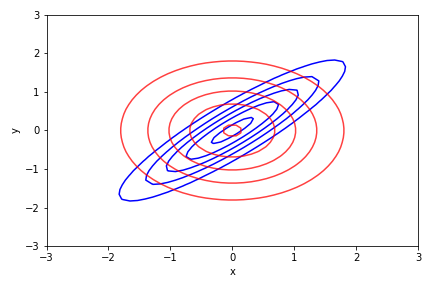
\includegraphics[width=0.45\textwidth]
		{figs/klil3b.png}}
\end{figure}
\end{block}
\end{frame}

\begin{frame}{Variational Inference}
\begin{block}{Mean field variational inference}
	Consider factorized proposals $q(\theta) = q(\theta_1)\ldots q(\theta_D)$.
	
	Training by coordinate descent 
	\begin{equation*}
	q^{*}_j(\theta_j;q_{-j}) \propto \exp \Ev_{\theta_{-j} \sim q_{-j}} [ \log \gu(\theta)].
	\end{equation*}
	
\end{block}
\begin{block}{Generic variational inference}
Uses stochastic gradient descent to find $q(\theta;\lambda)$.

REINFORCE: $\nabla \mathcal{L}(\lambda) = \Ev_{q(\theta;\lambda)} \left[ \left( \log \left( \frac{\gu(\theta)}{q(\theta;\lambda)}\right) + C\right) \nabla_{\lambda} \log q(\theta;\lambda) \right]$

Reparametrization: $\nabla \mathcal{L}(\lambda) = \nabla \left( \Ev_{r(\epsilon)} \left[\log \frac{ \gu(s(\epsilon;\lambda))}{q(s(\epsilon;\lambda);\lambda)}\right]\right) \approx \frac{1}{K} \sum_{i \in [K], \epsilon_i \sim r(\epsilon)} \nabla \left( \log \frac{ \gu(s(\epsilon;\lambda))}{q(s(\epsilon;\lambda);\lambda)} \right).$
\end{block}
\end{frame}

\begin{frame}{Variational Inference}
\begin{block}{Mixture of Gaussians}
$q_k(\theta;\lambda) = \sum_{i=1}^k w_i f_i(\theta) = \sum_{i=1}^k w_i \mathcal{N}(\theta;\mu_,\Sigma_i)$. Analytical mean and covariance. Samples can be easily generated.

Covariance parameterizations: 
\begin{itemize}
	\item $\Sigma_i = \text{diag}(\sigma_{i,1}^2,\ldots,\sigma_{i,D}^2)$
	\item $\Sigma_i = \u_i \u_i^T + \text{diag}(\sigma_{i,1}^2,\ldots,\sigma_{i,D}^2)$
\end{itemize}

Weights parameterizations $w_i(\nu_i) = \frac{\phi(\nu_i)}{\sum_{i=1}^k \phi(\nu_k)}$. $\phi$ can be:
\begin{itemize}
	\item $\phi(\nu) = \exp(\nu)$
	\item $\phi(\nu) = \text{softplus}(\nu) = \log(1+\exp(\nu))$
\end{itemize}
\begin{equation*}
\mathcal{L}(\lambda) = \sum_{i=1}^k w_i(\nu_i) \Ev_{\epsilon \sim \mathcal{N}(0,I)}\left[\log \frac{ \gu(s(\epsilon;\mu_i,\sigma_i))}{q_k(s(\epsilon;\mu_i,\sigma_i);\lambda)}\right]
\end{equation*}

\end{block}
\end{frame}

\begin{frame}{Variational Inference}
\begin{block}{Boosting mixtures}
Problem: no way to know how many mixtures is needed. Adding mixtures sequentially can become costly. One solution: boosting.
$q_{i-1}(\theta) = \sum_{j=1}^{i-1} w_j f_j(\theta)$

$q_{i}(\theta) = \sum_{j=1}^{i-1} (1-w_{i}) w_j f_j(\theta) + w_{i} f_i(\theta)$

How to find $w_{i}$ and $f_i(\theta) = \mathcal{N}(\theta;\mu_{i},\Sigma_{i})$?
\begin{itemize}
	\item Optimize jointly $\mathcal{L}_{i}(w_{i},\mu_{i},\Sigma_{i})$
	\item Seek good proposal $f_i(\theta)$ and optimize $\mathcal{L}_{i}(w_{i})$ via it's derivative
\begin{equation*}
\begin{split}
	\mathcal{L}'_{i}(w_{i}) & = \int \log (\gu(\theta)) (f_{i}(\theta) - q_{i-1}(\theta)) d\theta - \\
	& \qquad{} \int \log((1-w_{i}) q_{i-1}(\theta) + w_{i} f_{i}(\theta)) (f_i(\theta) - q_{i-1}(\theta)) d\theta.
\end{split}
\end{equation*}
\end{itemize}
\end{block}
\end{frame}

\begin{frame}{Variational Inference}
\begin{block}{Gradient boosting of mixtures}

\begin{equation*}
\begin{split}
f_i = \argmin_{f} \nabla D_{KL}(q_{i-1} || g) \cdot f = \argmin_{f} \int \log \frac{q_{i-1}(\theta)}{g(\theta)} f(\theta) d\theta.
\end{split}
\end{equation*}
Problem: degenerate solution. Needs regularization.

Maximization objective for mixture of Gaussians:
\begin{equation*}
\begin{split}
\text{RELBO}(\mu_i,\Sigma_i) = & \int \log(\gu(\theta)) \mathcal{N}(\theta|\mu_i,\Sigma_i) d\theta - \\
& \int \log(q_{i-1}(\theta)) \mathcal{N}(\theta|\mu_i,\Sigma_i) d\theta + \frac{\lambda}{4} \log |\Sigma|,
\end{split}
\end{equation*}
Estimated by the reparameterization trick.
\end{block}

\end{frame}

\begin{frame}{Variational Inference}
\begin{figure}
	\begin{algorithmic}[1]\label{vbalgorithm}
		\Procedure{VariationalBoosting}{$\log \gu,\mu_0$,$\Sigma_0$}
		\LineComment{$\mu_0,\Sigma_0$ the are initial boosting values}
		\State $w_0 := 1.0$
		\For{$t=1,...,T$}
		\State $\mu_{t},\Sigma_{t} := \argmax RELBO(\mu_{t},\Sigma_{t})$ \Comment{Using reparameterization}
		\State $w_{t} := \argmax \mathcal{L}_i(w_i)$ \Comment{Using $\mathcal{L}'_t(w_t)$ for gradient descent}
		\For{$j=0,...,t-1$}
		\State $w_{j} \gets (1-w_t)w_j$
		\EndFor
		\EndFor
		\State \Return $\{(\mu_t,\Sigma_t,w_t)\}_{t=1}^T$
		\EndProcedure
	\end{algorithmic}
\end{figure}
\end{frame}

\begin{frame}{Variational Inference}
\begin{block}{Variational Bayesian Monte Carlo (VBMC)}
$\mathcal{L}(\lambda) = 
 \int \log \gu(\theta) q(\theta;\lambda) d\theta - \int \log q(\theta;\lambda) q(\theta;\lambda) d\theta$
 
Use Bayesian Monte Carlo:
$\mathcal{L}_\mathcal{D}(\lambda) = 
\int \log \gu_\mathcal{D}(\theta) q(\theta;\lambda) d\theta - \int \log q(\theta;\lambda) q(\theta;\lambda) d\theta$

\begin{block}{}
\begin{equation*}
\begin{split}
\text{Maximize } \Ev[\mathcal{L}_\mathcal{D}(\lambda)] & = M(\lambda) + \mathbf{z}^T \mathbf{w} - \int \log q(\theta;\lambda) q(\theta;\lambda) d\theta\\
\mathbf{w} & = K^{-1} \mathbf{y} \\
M(\lambda) & = \int m(\theta) q(\theta;\lambda) d\theta \\
\mathbf{z}_i & = \int k(x,x_i) q(\theta;\lambda) dx.
\end{split}
\end{equation*}

\end{block}
\end{block}
\end{frame}

\begin{frame}{Variational Inference}
\begin{block}{Mean function}
$m(\theta) = 0$: $\log \gu_\mathcal{D}(\theta)$ is not a log probability

Principled solution: $m(\theta) = -\frac{1}{2} \sum_{i=1}^D \frac{(\theta_i - c_i)^2}{l_i^2}$. Lends analytical $M(\lambda)$.

Ad-hoc solution: $m(\theta) = C$, with $C$ being a large negative constant.
\end{block}

\begin{block}{Active evaluation}
Just as in BMC, it is possible to do active evaluation.
Some options:
\begin{itemize}
	\item $\alpha^\mathcal{D}_{\text{US}}(\theta_{N+1}) = k_\mathcal{D}(\theta_{N+1},\theta_{N+1}) q_k(\theta_{N+1};\lambda)^2.$
	\item $\label{prospective_vbmc}
	\alpha^\mathcal{D}_{\text{PROP}}(\theta_{N+1}) = k_\mathcal{D}(\theta_{N+1},\theta_{N+1}) \exp(m_\mathcal{D}(\theta_{N+1}))q_k(\theta_{N+1};\lambda)^2$
\end{itemize}
\end{block}
\end{frame}

\section{Boosted Variational Bayesian Monte Carlo}
\begin{frame}{Boosted Variational Bayesian Monte Carlo}
\begin{block}{BVBMC}
BVBMC = VBMC + boosting + small changes
\end{block}
\begin{block}{BMC in boosted variational inference}
\begin{equation*}
\begin{split}
\text{RELBO}_\mathcal{D}(\mu_i,\Sigma_i) = & \int \Ev[\log \gu_\mathcal{D}(\theta)] \mathcal{N}(\theta|\mu_i,\Sigma_i) d\theta - \\ &\int \log(q_{i-1}(\theta)) \mathcal{N}(\theta|\mu_i,\Sigma_i) d\theta
+ \frac{\lambda}{4} \log |\Sigma_i|
\end{split}
\end{equation*}
\begin{equation*}
\begin{split}
\mathcal{L}_{i,\mathcal{D}}(w) = & \int \log \gu_\mathcal{D}(\theta)
((1-w_{i}) q_{i-1}(\theta) + w_{i} f_{i}(\theta)) d\theta - \\
& \int \log ((1-w_{i}) q_{i-1}(\theta) + w_{i} f_{i}(\theta)) ((1-w_{i}) q_{i-1}(\theta) + w_{i} f_{i}(\theta)) d\theta \\
\end{split}
\end{equation*}
\end{block}
\end{frame}

\begin{frame}{Boosted Variational Bayesian Monte Carlo}
\begin{block}{Practical considerations}
\begin{itemize}
	\item RELBO stabilization
	\begin{equation*}
	\text{RELBO}^{\delta_D}_\mathcal{D}(\mu_i,\Sigma_i) = \int \log \left(\frac{r_\mathcal{D}(\theta)}{q_{i-1}(\theta)+\delta_D} \right) \mathcal{N}(\theta;\mu_i,\Sigma_i) d \theta + \log |\Sigma_i|.
	\end{equation*}
	\item Output scaling
	\begin{equation*}
	\tilde{y}_i = (y_i-m_y)/\sigma_y, \, \tilde{\mathcal{D}} = \{x_i,\tilde{y}_i\}, \,\sigma_y \log g_\mathcal{\tilde{D}}(x) + \mu_y
	\end{equation*}
	\item Component pruning: discard negligible components
	\item Initialization: either large covariance or maximize ELBO for first Gaussian component.
	\item Mean function: $m(\theta) = C$ found to be more stable.
\end{itemize}

\end{block}

\end{frame}

\begin{frame}
\begin{block}{Practical considerations}
	\begin{itemize}
	\item Periodic joint parameter updating: sometimes maximize $\Ev[\mathcal{L}_\mathcal{D}(\lambda)]$ for all parameters in $\sum_{i=1}^k w_k \mathcal{N}(\theta;\mu_k,\Sigma_k)$.
	\item Product of Matern kernels:
	\begin{equation*}
	 k_{\text{PMat},\nu}(x,x';\theta,l) = \theta \prod_{d=1}^D k_{\text{Matern},\nu}(|x_i-x_i'|;l_d).
	\end{equation*}
	Is integrated in BVBMC by Gauss-Hermite quadrature. Found to be more stable than the SQE kernel.
	\item More acquisition functions:
	\begin{equation*}
	\alpha^\mathcal{D}_{MMLT}(x_{m+1}) = e^{2 m_\mathcal{D}(x) + k_\mathcal{D}(x,x)} \left(e^{k_\mathcal{D}(x,x')}-1\right).
	\end{equation*}
	\begin{equation*}
	\alpha^\mathcal{D}_{MMLT_P}(x_{m+1}) = e^{2 m_\mathcal{D}(x) + k_\mathcal{D}(x,x)} \left(e^{k_\mathcal{D}(x,x')}-1\right)q_k(\theta_{N+1};\lambda)^2.
	\end{equation*}
	\end{itemize}
\end{block}
\end{frame}

\section{Experiments}
\begin{frame}
\begin{block}{1-d mixture of Gaussians}
\begin{figure}
	\centering
	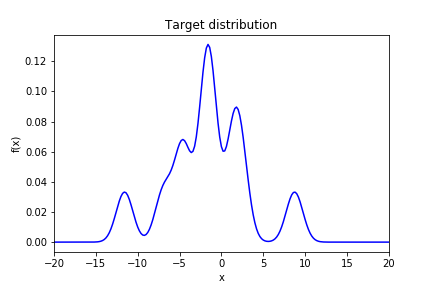
\includegraphics[width=0.6\linewidth]{figs/targetexil1a.png}
\end{figure}
\begin{displaymath}
f(x) = \sum_{i=1}^{12} w_i \mathcal{N}(x;\mu_i,\sigma^2_i),
\end{displaymath}
\centering{$w_i = \frac{1}{12}$, $\mu_i \sim \mathcal{N}(0,\sqrt{5})$, $\sigma^2_i = 1$}.
\end{block}
\end{frame}

\begin{frame}

\end{frame}


\end{document}

